\section{Kiến trúc hệ thống và cấu trúc module mã nguồn}
\label{sec:kien_truc_he_thong}

\subsection{Sơ đồ khối luồng xử lý dữ liệu tổng thể}

Hệ thống phát hiện vết dầu loang trên ảnh SAR được thiết kế theo kiến trúc quy trình tuần tự 2 giai đoạn khép kín, gồm 6 khối chức năng được liên kết chặt chẽ như minh họa trên Hình~\ref{fig:pipeline_overview_ch3}. 

\begin{figure}[!htbp]
\centering
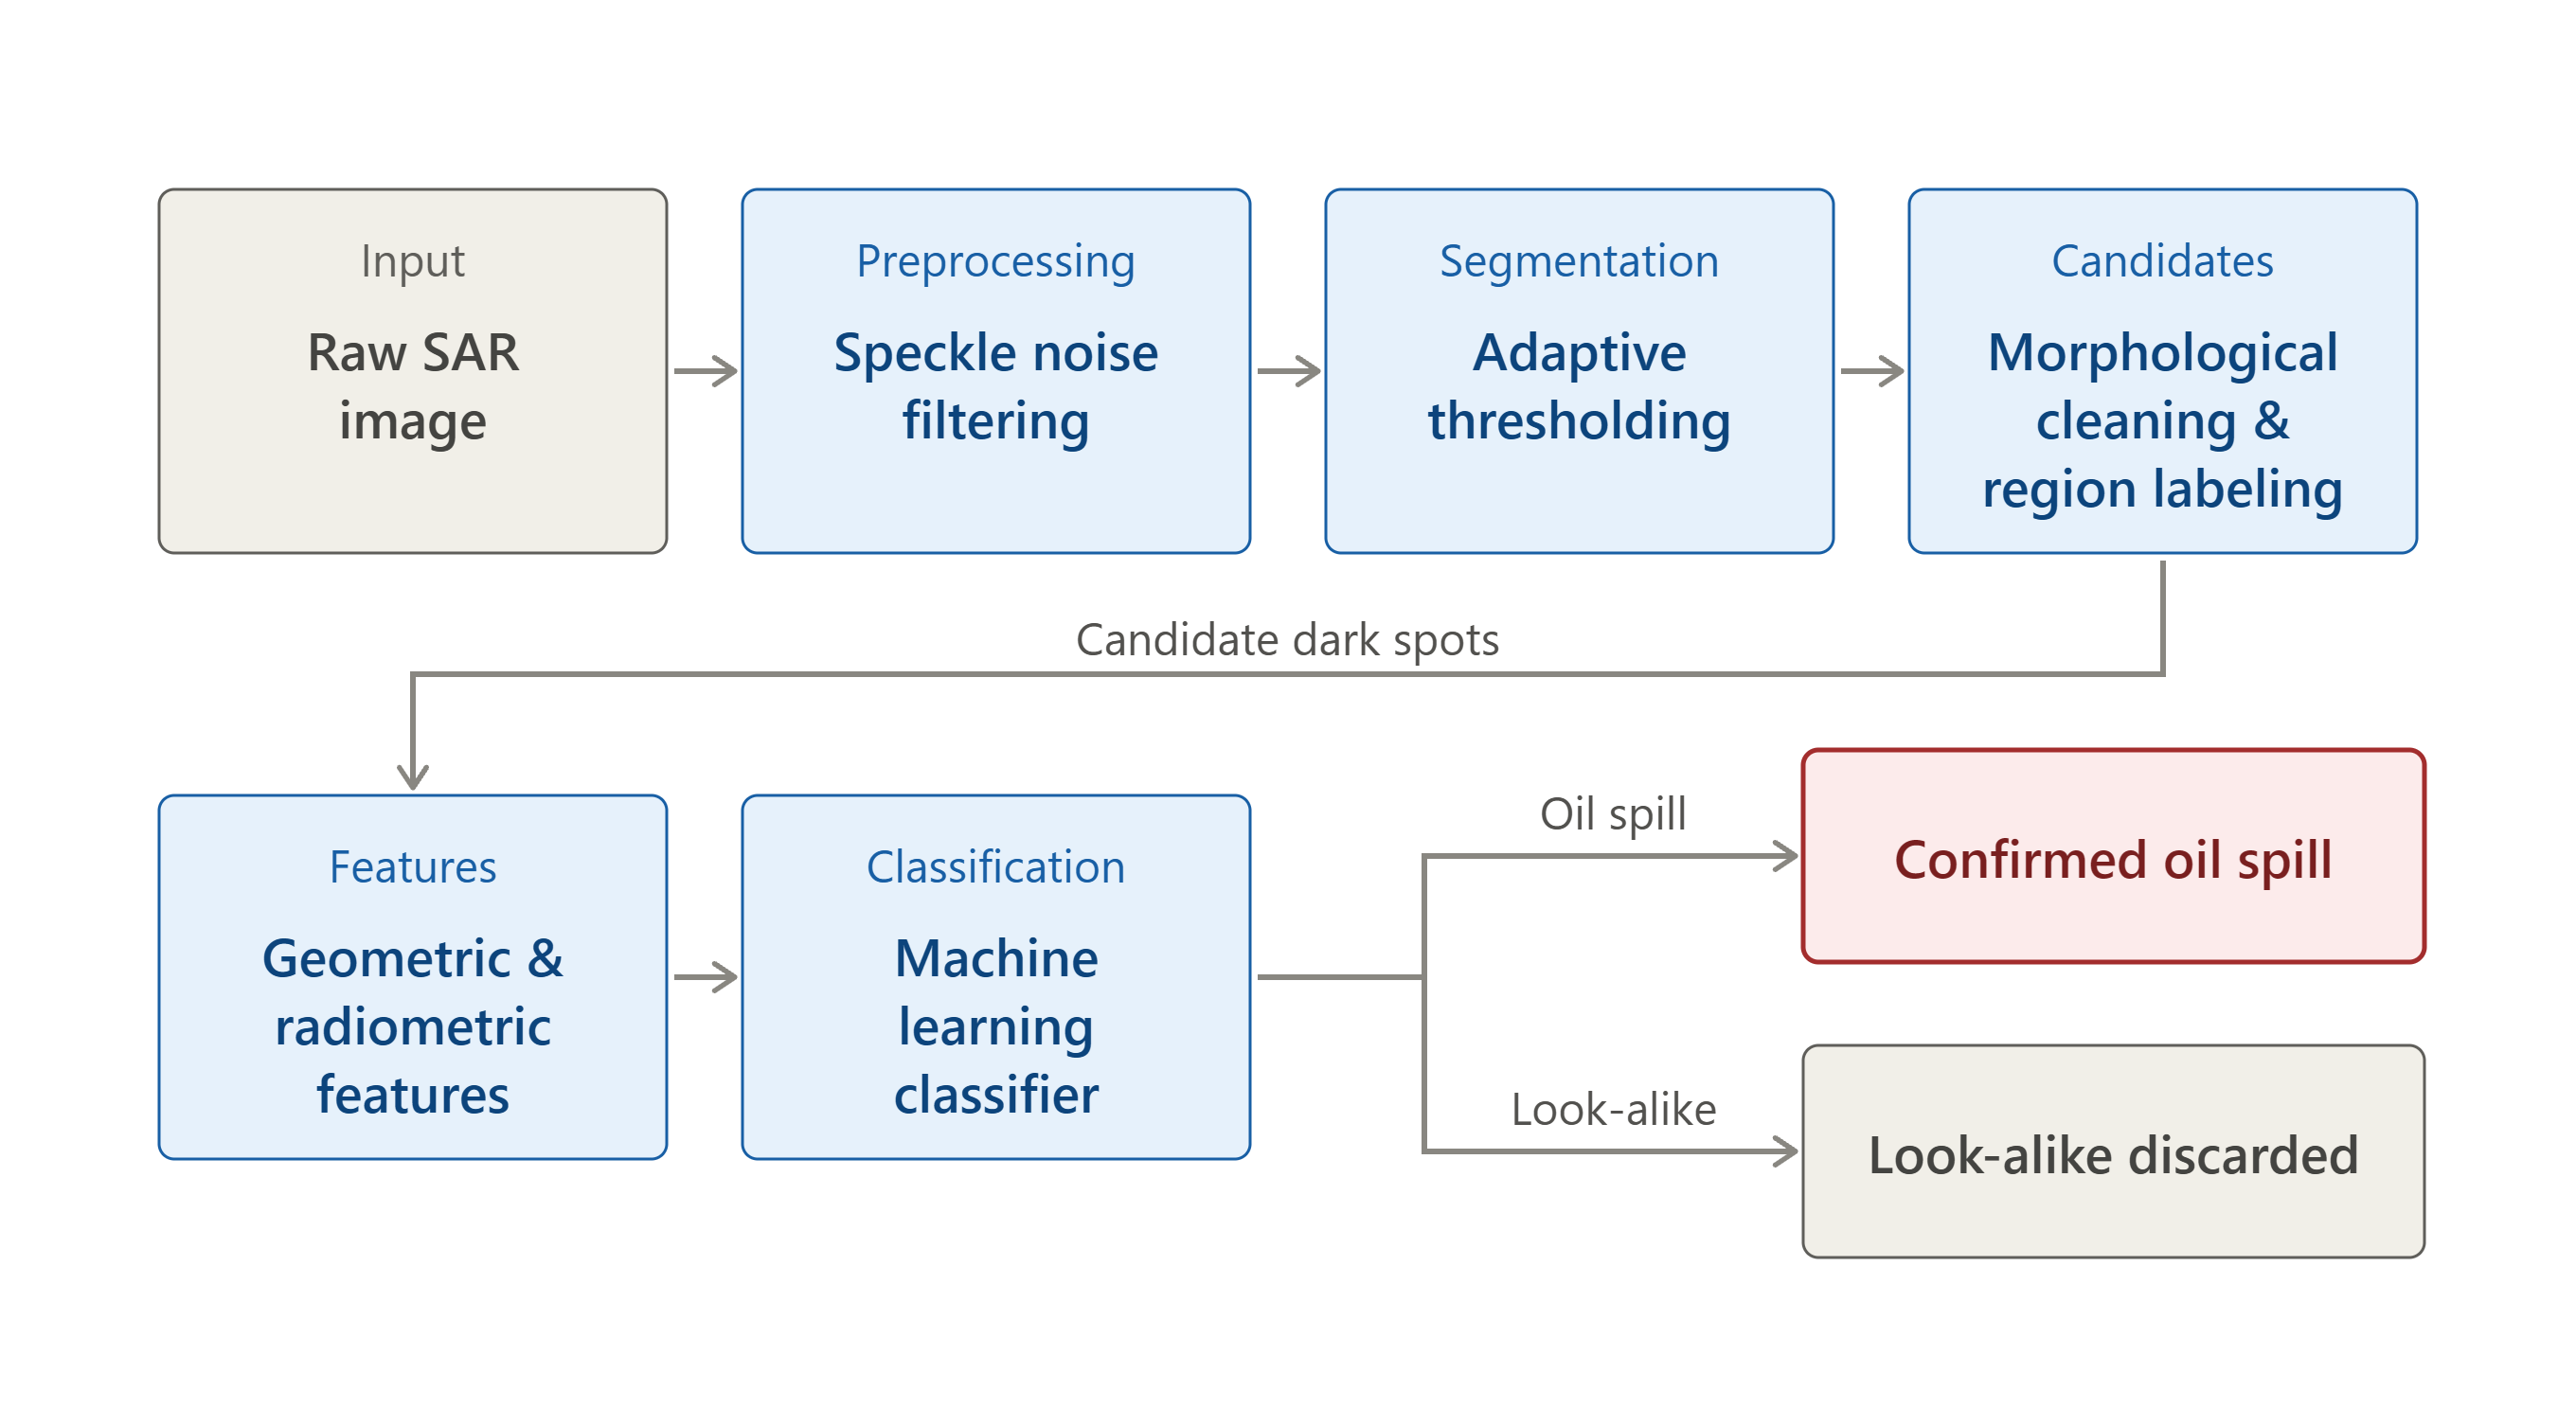
\includegraphics[width=0.88\linewidth, height=0.28\textheight, keepaspectratio]{figures/sar_oil_spill_detection_pipeline.png}
\caption{Kiến trúc 2 giai đoạn (6 khối chức năng) của quy trình phát hiện vết dầu loang từ ảnh SAR.}
\label{fig:pipeline_overview_ch3}
\end{figure}

Luồng biến đổi dữ liệu giữa các khối được quy định cụ thể qua Bảng~\ref{tab:luong_du_lieu_pipeline}:
\begin{enumerate}
    \item \textbf{Giai đoạn 1 (Tạo vùng ứng viên):} Chuyển đổi ảnh thô $I \in [0, 1]$ sang $K$ vùng tối ứng viên rời rạc $\{\Omega_1, \dots, \Omega_K\}$ qua lọc Lee MMSE $\mathcal{O}(HW)$, phân ngưỡng Otsu, lọc diện tích $A_{\min} = 64$ và gán nhãn liên thông 8 hướng.
    \item \textbf{Giai đoạn 2 (Phân loại vùng):} Trích xuất vector 8 đặc trưng $\mathbf{x}_i \in \mathbb{R}^8$ và thẩm định bằng LinearSVM; các vùng có $\mathbf{z}_i^T \mathbf{w} \le 0$ bị loại bỏ, các vùng có $\mathbf{z}_i^T \mathbf{w} > 0$ được giữ lại trong mặt nạ dự đoán $\hat{M}$.
\end{enumerate}

\begin{table}[!htbp]
\centering
\small
\caption{Đầu vào, phép toán và kiểu dữ liệu đầu ra của các bước trong pipeline đã khóa.}
\label{tab:luong_du_lieu_pipeline}
\begin{tabular}{|c|p{2.8cm}|p{4.6cm}|p{4.0cm}|}
\hline
\textbf{Bước} & \textbf{Dữ liệu đầu vào} & \textbf{Thuật toán thực thi} & \textbf{Dữ liệu và kiểu đầu ra} \\ \hline
\textbf{1. Tiền xử lý} & Ảnh PNG 8-bit $[0, 255]$ & Ép kiểu và chia cho $255.0$ & Mảng thực $\texttt{float64} \in [0, 1]$ \\ \hline
\textbf{2. Lọc đốm} & Mảng ảnh mức xám & Lọc Lee MMSE $7 \times 7$ ($L=4$) qua bảng tích lũy SAT & Ảnh làm mượt $I_f \in [0, 1]$ \\ \hline
\textbf{3. Phân đoạn} & Ảnh làm mượt $I_f$ & Phân ngưỡng toàn cục Otsu 256 bin ($t^*$) & Mặt nạ nhị phân thô $\texttt{bool}$ \\ \hline
\textbf{4. Hậu xử lý} & Mặt nạ nhị phân thô & Lọc diện tích $A \ge 64$ và gán nhãn liên thông 8 hướng & Bản đồ nhãn $\texttt{int32}$, $K$ vùng ứng viên $\{\Omega_i\}$ \\ \hline
\textbf{5. Đặc trưng} & Bản đồ nhãn và $I_f$ & Trích xuất 4 hình học và 4 bức xạ/biên theo hộp bao lề 5px & Ma trận đặc trưng $K \times 8$ và danh sách vùng \\ \hline
\textbf{6. Phân loại} & Ma trận đặc trưng & Chuẩn hóa Z-score và suy luận LinearSVM ($C=10$) & Mặt nạ nhị phân cuối $\hat{M}$, overlay và JSON vùng \\ \hline
\end{tabular}
\end{table}

\subsection{Cấu trúc thư mục mã nguồn và hệ thống sổ tay thực nghiệm}

Toàn bộ mã nguồn được tổ chức module hóa trong thư mục \texttt{src/sar\_oil/}:
\begin{itemize}
    \item \texttt{data.py}: Đọc cặp ảnh--mask, kiểm kê mã băm (\texttt{manifest.json}) và phân chia tập Train / Validation / Test.
    \item \texttt{core.py}: Các thuật toán xử lý ảnh tự cài đặt bằng NumPy thuần (SAT, lọc Lee, Otsu, Niblack, hình thái học, CCL 8 hướng, 8 đặc trưng vùng).
    \item \texttt{models.py}: Các bộ phân loại tự cài đặt từ đầu (CART theo tiêu chuẩn Gini và LinearSVM tối ưu bằng NAG).
    \item \texttt{pipeline.py} \& \texttt{evaluation.py}: Luồng suy luận độc lập (không nhận nhãn Ground Truth) và đánh giá ghép cặp một-một Hungarian ở ngưỡng $\IoU \ge 0.5$.
    \item \texttt{reference.py}, \texttt{verification.py} \& \texttt{experiments.py}: Hàm tham chiếu thư viện chuẩn (\texttt{SciPy}, \texttt{scikit-image}, \texttt{scikit-learn}), kiểm thử 118 ca biên và quét lưới $110 \times 729$ cấu hình.
\end{itemize}

Hệ thống cung cấp giao diện dòng lệnh \texttt{scripts/sos.py} cùng 5 sổ tay Jupyter Notebook tương tác (\texttt{01\_data\_and\_ground\_truth.ipynb} đến \texttt{05\_final\_pipeline.ipynb}) để trực quan hóa từng bước và tái lập kết quả thực nghiệm.
